\documentclass{endm}
\usepackage{endmmacro}
\usepackage{graphicx}

\usepackage{amssymb,amsmath,latexsym}
\usepackage[varg]{pxfonts}
%%%%%% ENTER ADDITIONAL PACKAGES
%\usepackage{graphics}
\usepackage{pst-all}
\usepackage{graphicx}
\usepackage{amsmath,amsfonts}
\usepackage{amssymb} % ADDED
\usepackage{times}
\usepackage{latexsym}
\usepackage{fancybox}
\usepackage{algorithm}
%\usepackage{algorithmic}
\usepackage{algorithmicx}
\usepackage{algpseudocode}
\usepackage{setspace}
\usepackage{courier}
\usepackage{verbatim}
\usepackage{hhline}
\usepackage{etex}
\usepackage{tikz}
\usetikzlibrary{calc,arrows,automata}
\usetikzlibrary{matrix,positioning,arrows,decorations.pathmorphing,shapes}
\usetikzlibrary{shapes,snakes}
\usepackage{graphicx}

\usepackage{mathrsfs}
\usepackage[a4paper, total={6in, 8in}]{geometry}
\usepackage{titlesec}
\titlespacing{\subsection}
    {1pt}{1ex}{0ex}
%---------------
\usepackage{subfigure}
\usepackage{mathtools}
\usepackage{booktabs}
\usepackage{hyperref}

\tolerance=1
\emergencystretch=\maxdimen
\hyphenpenalty=10000
\hbadness=10000


\floatname{algorithm}{Algorithm}


\def\lastname{Toyos}

\begin{document}

% DO NOT REMOVE: Creates space for Elsevier logo, ScienceDirect logo% and ENDM logo
\begin{verbatim}
\end{verbatim}
\vspace{2.5cm}

\begin{frontmatter}

\title{Obligatorio 1 - Implementación del método de “Residuo Mínimo Generalizado” (GMRES)}

\subtitle{Grupo 36}

\author{Guillermo Daniel Toyos Marfurt (5139879-9),}
\author{Juan Jos\'e Mangado Esteves (5535227-0),}
\author{Martín Sebastián Piñeyro Olivera (5043446-7),}
\author{Ricardo Alejandro Fasanello Guillermo (4763979-9)}

\address{Tutor: Juan Piccini}
\address{M\'etodos Num\'ericos 2020\\ Instituto de Matem\'atica y Estad\'istica\\ Facultad de Ingenier\'ia. Universidad de la Rep\'ublica\\ Montevideo, Uruguay}
\begin{abstract}
\setlength{\parindent}{12pt}
Se estudia la resolución de sistemas lineales $Ax=b$ donde $A$ es una matriz dispersa utilizando el método iterativo de Residuo Mínimo Generalizado (GMRES). Para ello se implementa este método y se prueba la complejidad computacional de su implementación. Adicionalmente se encuentra una cota teórica dependiente de los valores propios de A. La cual asegura la convergencia y rapidez del método si el cociente entre el radio y el centro del disco donde los valores propios caen es pequeño. También se estudia experimentalmente el comportamiento de GMRES con matrices dispersas aleatorias y se presentan distintas gráficas que caracterizan el comportamiento del método. El informe finaliza con pruebas de tiempo medio de ejecución que comparan el método GMRES con el comando \textit{“contrabarra”} de \textit{Octave} mostrando la superioridad de GMRES a medida que la dimensión de A es cada vez más grande.
%El objetivo es resolver un sistema lineal $Ax = b$ para el caso donde $A \in \mathbb{R}^{n \times %n}$ es
%una matriz dispersa, $b \in \mathbb{R}^{n}$, y x es un vector perteneciente al subespacio de %Krylov.
%Implementamos el metodo GMRES (junto con los m\'etodos que utiliza), dada su eficiencia sobre %dichas matrices por sobre los m\'etodos tradicionales.\\
%x El algoritmo es mas eficiente para matrices particulares (ESPARSAS ...) que los metodos %tradicionales 
\end{abstract}

\begin{keyword}
Sistemas lineales, Métodos Iterativos, GMRES, Matrices dispersas
\end{keyword}

\end{frontmatter}


4\section{Introducci\'on}\label{intro}
El problema de resolver un sistema $Ax=b$ es uno de los problemas fundamentales del álgebra lineal. \'Este problema, a priori, es  f\'acil de resolver; se podr\'ia usar un m\'etodo de resoluci\'on directo, como puede ser el m\'etodo de Escalerizaci\'on Gaussiana, y as\'i obtener los valores de las inc\'ognitas.\\

El problema aparece cuando la cantidad de incógnitas (la dimensión de A) es muy grande, ya que los métodos directos como la escalerización Gaussiana o descomposición LU no solo necesitan realizar demasiadas operaciones sino también requieren almacenar matrices auxiliares de tamaño prohibitivo. Por ello se idearon los métodos iterativos, estos son un tipo de método el cual se basa en aproximar sucesivamente la solución en cada iteración, mejorando la precisión conforme avanzamos en la iteración. Existen diversos métodos iterativos, los cuales dependiendo de las características del problema se “acercan” más rápido que otros. En este informe se estudiará el método iterativo GMRES propuesto en 1986 por Youcef Saad y Martin H. Schultz \cite{GMRES} . GMRES resulta particularmente eficiente para resolver problemas donde el número de incógnitas es enorme, pero estás aparecen contadas veces en cada ecuación. Esto es cuando A es una matriz dispersa.\\

El informe realiza los siguientes aportes:
\begin{itemize}
    \item Se proporciona una síntesis de la metodología que utiliza GMRES y como se implementa el mismo
    \item  Análisis de complejidad computacional de las distintas partes del algoritmo GMRES
    \item Obtención una cota teórica de la norma del residuo relativo. Generando un criterio de convergencia y rapidez de esta.
    \item Un estudio experimental con matrices dispersas de distribución aleatoria para confirmar la cota del residuo propuesta y la velocidad de convergencia de GMRES
    \item Comparación de tiempos de ejecución de la implementación de GMRES con el comando \textit{“contrabarra”} de \textit{Octave}
\end{itemize}
El informe se organiza de la siguiente manera. La sección (3) trata sobre la metodología, implementación y complejidad de GMRES. La sección (4) presenta los resultados del análisis experimental junto al desarrollo de la cota teoría para la convergencia del método. Finalmente, la sección (5) presenta las conclusiones halladas.  





%El objetivo de este informe consiste en mostrar e implementar una herramienta para la resoluci\'on de sistemas de ecuaciones lineales; en particular, el m\'etodo de Residuo M\'inimo Generalizado, o GMRES por sus siglas en Ingl\'es.\\

%Un m\'etodo iterativo es un m\'etodo que se basa en aproximar sucesivamente la soluci\'on de un sistema de ecuaciones lineales, mejorando la precisi\'on conforme iteramos el m\'etodo.\\

%El metodo Generalized Minimal Residual (GMRES) propuesto en 1986 por Youcef Saad y Martin H. Schultz \cite{GMRES} es un m\'etodo iterativo que utiliza el algoritmo de Arnoldi (un método para obtener una base ortonormal del subespacio de Krylov), y la descomposición QR de una matriz de Hessenberg, calculada mediante rotaciones de Givens, para luego usarla para resolver Problemas de M\'inimos Cuadrados Lineales. En la metodolog\'ia, se explicar\'a con detalle cada una de las partes.\\

%Este m\'etodo se destaca de otros m\'etodos iterativos que usan subespacios de Krylov, pues no es necesario que la matriz A sea definida positiva ni sim\'etrica. El m\'etodo GMRES es m\'as eficiente que los m\'etodos tradicionales, y otros m\'etodos del estilo, sobre todo para matrices esparsas (matrices con grandes cantidades de coeficientes nulos)\\

%El informe se organiza de la siguiente manera:

%\begin{enumerate}
%    \item Problema a resolver.
%    \item Qu\'e utiliza el m\'etodo GMRES.
%    \item Se presenta el m\'etodo.
%    \item Se muestra el orden del algoritmo utilizado.
%    \item Se llega a una cota teorica del residuo.
%    \item Se realizan pruebas experimentales.
%    \item Se muestra la superioridad de GMRES sobre los demas m\'etodos.
%    \item Presentar las conclusiones.
%\end{enumerate}
\clearpage
\section{Problema a resolver}\label{Problem}
Dada una matriz $A \in \mathbb{M}^{n \times n}$, un vector $b \in \mathbb{M}^{n \times 1}$ se quiere hallar un vector $x \in \mathbb{M}^{n \times 1} : Ax=b$. Queremos resolver este problema cuando la matriz $A$ y el vector $b$ son dispersos, ya que es en estas condiciones que el algoritmo GMRES resulta eficiente.
%Se tiene un sistema de ecuaciones lineales $Ax = b$, donde $A \in \mathbb{R}^{n \times n}, x, b \in \mathbb{R}^{n}$. Este problema, a priori, es  f\'acil de resolver; se podr\'ia usar un m\'etodo de resoluci\'on directo, como puede ser el m\'etodo de Escalerizaci\'on Gaussiana, y as\'i obtener los valores de las inc\'ognitas. Para peque\~{n}os vol\'umenes de datos, este m\'etodo no supondr\'ia ning\'un inconveniente, pero si tenemos un sistema de ecuaciones con una cantidad grande de inc\'ognitas (y datos de entrada), ser\'ia un problema, ya de por s\'i costoso de resolver mediante el uso de computadoras (impensable resolver a mano). Y esto se debe a que la cantidad de operaciones que es necesario ejecutar para aplicar el algoritmo de Escalerizaci\'on Gaussiana, ronda el $O(n^3)$. Si tuvi\'eramos un sistema de mil ecuaciones con mil inc\'ognitas, suponiendo que nuestra computadora hace mil c\'alculos por segundo, este problema tardar\'ia aproximadamente $11.6$ d\'ias en resolverse.\\

%Afortunadamente, \'este m\'etodo no es el \'unico que existe para la resoluci\'on de este tipo de problemas. Existen otros m\'etodos, tanto directos como iterativos, y este trabajo har\'a un enfoque en uno de los \'ultimos. Se busca implementar GMRES ya que, si bien no nos dar\'a la soluci\'on exacta, s\'i nos dar\'a una soluci\'on aproximada, cuyo error se puede despreciar, y en una menor cantidad de pasos.\\

\section{Metodolog\'ia}\label{AA}
A continuaci\'on, se presenta una síntesis de la maquinaria matemática que utiliza GMRES para su implementación.\\

%\begin{enumerate}
 %   \item Rotaciones de Givens
  %% \item M\'inimos Cuadrados con QR
   % \item Ortogonalizaci\'on con Gram-Schmidt
    %\item Base ortonormal del Subespacio Krylov
%\end{enumerate}
%listado de temas junto con sus respectivos desarrollos, con el fin de tener un adecuado entendimiento sobre los m\'etodos aplicados al algoritmo de GMRES que se ver\'a al final de \'esta secci\'on.
\subsection{Rotaciones de Givens}\label{givens}

Las rotaciones de Givens son transformaciones lineales ortogonales definidas como
\begin{equation*}G(i, k, \theta) = \begin{pmatrix}
1 & \cdots & 0 & \cdots & 0 & \cdots & 0\\
\vdots & \ddots & \vdots & & \vdots & & \vdots\\
0 & \cdots & c & \cdots & s & \cdots & 0\\
\vdots & & \vdots & \ddots & \vdots & & \vdots\\
0 & \cdots & -s & \cdots & c & \cdots & 0\\
\vdots & & \vdots & & \vdots & \ddots & \vdots\\
0 & \cdots & 0 & \cdots & 0 & \cdots & 1
\end{pmatrix}
\end{equation*}\\
Específicamente sus entradas no nulas se definen con $i>J$ en:
\begin{align*}
 g_{kk} = 1, \  (k  \not=i \land k\not=j) \\
 g_{kk} = c, \ (k=j \lor k=i) \\
 g_{ji} = -g_{ij} = s
\end{align*}
$G^t$ representa rotaciones antihorarias sobre el plano $(i,j)$ de un espacio de $n>1$ dimensiones de $\theta$ radianes: $G(i, j, \theta)^{t}$. Podemos escoger los parámetros $c$ y $s$ con el objetivo de anular una de las entradas de un vector $x \in \mathbb{R}^n$. Suponiendo que queremos anular las entradas $x_{i}$ y $x_j$ basta asignar los parámetros con:
\begin{equation*}
c = \frac{x_i}{\sqrt{x_{i}^{2} + x_{j}^{2}}}, \hspace{1cm} s = \frac{-x_j}{\sqrt{x_{i}^{2} + x_{j}^{2}}}
\end{equation*}\\
Existen varias formas de calcular $s$ y $c$. Nuestra implementación de GMRES utiliza el algoritmo [5.1.3]\cite{matrixcomp} que reduce el error de redondeo al evitar la división directa por la norma de $x_{i}$ y $x_j$. De todas maneras el cálculo de los parámetros de una rotación de Givens es $\mathcal{O}(1)$.


\subsection{QR de una matriz de Hessenberg aplicando Givens}\label{QRHgivens}

Dada una matriz $H \in \mathbb{R}^{(n+1) \times n}$, $H$ se considera "Hessenberg superior" cuando los valores de la subdiagonal inferior son todos nulos.\'Esto mismo tambi\'en se aplica para matrices $n\times n$. \\
Podemos utilizar rotaciones de Givens para realizar la descomposici\'on QR de $H$ de forma eficaz.Por ejemplo, sea $H \in \mathbb{R}^{(n+1) \times n}$, con $n = 3$ y entradas $\times$ arbitrarias: 
\begin{equation*}
    H = \begin{pmatrix}
            \times & \times & \times\\
            \times & \times & \times\\
            0      & \times & \times\\
            0      & 0      & \times\\
        \end{pmatrix}
\end{equation*} donde las $\times$ son entradas arbitrarias.
Para escalerizar $H$ (y por ende hallar su descomposici\'on $QR$), se le va aplicando rotaciones de Givens $G(i,j,\theta)$ de forma iterativa, donde $G(j,i,\theta)$ anula el elemento (i,j)-\'esimo de $H$:\\

\begin{multline*}
    G(1,2,\theta_{1})^{T}\cdot H = \begin{pmatrix}
            \times & \times & \times\\
            0      & \times & \times\\
            0      & \times & \times\\
            0      & 0      & \times\\
        \end{pmatrix}
    =     G(2,3,\theta_{2})^{T}\cdot G(1,2,\theta_{1})^{T}\cdot H = 
    \begin{pmatrix}
            \times & \times & \times\\
            0      & \times & \times\\
            0      & 0      & \times\\
            0      & 0      & \times\\
        \end{pmatrix} = \\
    G(3,4,\theta_{3})^{T}\cdot G(2,3,\theta_{2})^{T}\cdot G(1,2,\theta_{1})^{T}\cdot H = \begin{pmatrix}
            \times & \times & \times\\
            0      & \times & \times\\
            0      & 0      & \times\\
            0      & 0      & 0     \\
        \end{pmatrix} = R
\end{multline*}

Sí denominamos al producto de las rotaciones de Givens transpuestas como $Q^T$, se concluye el c\'omputo para la descomposici\'on $QR$ de $H$.\\
Seg\'un Golub y Van Loan (2013)\cite{matrixcomp}, el algoritmo para el proceso descripto anteriormente requiere alrededor de $n^2 \ flops$. Si bien cuándo $H$ es de Hessemberg no hay una ventaja evidente en la cantidad de operaciones entre utilizar rotaciones de Givens y Escalerización Gaussiana (el cual es $\mathcal{O}(n^2)$ para matriz  de Hessenberg), como este último realiza una cantidad de divisiones sobre las entradas mucho mayor va a tener más propagación de error. Especialmente cuando los valores de las entradas son pequeños. Además, las rotaciones de Givens eliminan la preocupación del pívot nulo. Simplificando la implementación.

%Seg\'un Golub y Van Loan (2013)\cite{matrixcomp}, el algoritmo para el proceso descripto anteriormente requiere alrededor de $3n^2 flops$ , lo cual resulta ser m\'as eficiente que la Escalerizaci\'on Gaussiana, que por resultados vistos en el te\'orico del curso se sabe que requiere $O(n^3) flops$.

\subsection{M\'inimos Cuadrados con QR} \label{mcqr}

Se desea resolver el siguiente Problema de M\'inimos Cuadrados Lineal. Hallar $x \in \mathbb{R}^m$ que minimice $\|H x - c\|_{2}^2$, con $H \in \mathbb{R}^{(m+1) \times m}, c \in \mathbb{R}^{m+1}$.

\begin{equation*}
    \min_{x \in \mathbb{R}^m} \|H x - c\|_2^2
\end{equation*}

Tenemos que $R = Q^{T}H$, con $R$ matriz triangular superior. $Q^{-1} = Q^{T}$. Utilizando este hecho junto con la proposición [4.3.2]\cite{notasteo}: $||QX||_2=||X||_2$ tenemos que:

\begin{multline*}
    \min_{x \in \mathbb{R}^m} \|H x - c\|_2^2 = \min_{x \in \mathbb{R}^m} \|QR x - c\|_2^2 = \min_{x \in \mathbb{R}^m} \|RX - Q^tc\|_2^2=\min_{x \in \mathbb{R}^m}\|R_1 x - (Q^tc)_1\|_2^2 + \|(Q^tc)_2\|_2^2
\end{multline*}

Separando $R$ en $R_1$ (matriz triangular superior cuadrada formada por las primeras $m$ filas de $R$) y escribiendo $(Q^tc) \in \mathbb{R}^m+1$ como $(Q^tc)_1 \in \mathbb{R}^m, \ (Q^tc)_2 \in \mathbb{R}^{m+1-m}$ como los vectores formados por los primeros $m$ y $m+1-m$ elementos de $Q^tc$ respectivamente. Como $ \|(Q^tc)_2\|_2^2$ no depende de $X$ el problema se traduce a resolver el sistema determinado $R_1 X = (Q^tc)_1$. Como $R_1$ es triangular superior, $x$ se obtiene haciendo sustituci\'on hacia atr\'as.\\

\textbf{Ejemplo Solicitado:} Probamos el método implementado con las siguientes matrices $H$ y $c$:
\begin{equation*}
    H = \begin{pmatrix}
        2 & 0 & 1 & 5\\
        -3 & 2 & -6 & 4\\
        0 & 4 & 7 & 1\\
        0 & 0 & -2 & 0\\
        0 & 0 & 0 & 6\\
    \end{pmatrix}, \
    c = \begin{pmatrix}
        3\\
        0\\
        0\\
        0\\
        0
    \end{pmatrix}
\end{equation*}\\
Obteniendo como resultado el vector solución $X^t \approx (1,398 \ 0,698 \ -0,3936 \ 0,060)$. Ejecutando el comando $H \setminus c$ en \textit{Octave} obtenemos exactamente los mismos resultados. Esto es esperado dado que este comando busca la solución de mínimos cuadrados si la matriz no es cuadrada\cite{octavelinalg}.

\subsection{Ortogonalizaci\'on con Gram-Schmidt} \label{ortgs}

El proceso de ortogonalizaci\'on de Gram-Schmidt es un m\'etodo utilizado principalmente en \'algebra lineal y an\'alisis num\'erico el cual toma como entrada un conjunto de vectores no ortogonales y linealmente independientes, y retorna una base ortonormal.\\

Dada una matriz $A = \big(a_1 , \dots , a_n \big) \in \mathbb{R}^{m \times n}$ tal que $m \geq n$,
$rango(A) = n$ y sus columnas $a_1, \dots , a_n$ son linealmente independientes entre s\'i, se puede
aplicar Gram-Schmidt para hallar su descomposici\'on $QR$ fina $Q_1 R_1$, donde $Q = \big(Q_1,Q_2 \big) \in \mathbb{R}^{m \times m}$ ($Q_1$ son sus primeras n columnas, y $Q_2$ sus \'ultimas $m - n$) ,
$R \in \mathbb{R}^{m \times n}$ tal que sus \'ultimas $m-n$ filas son nulas ,y $R_1$ es el mismo $R_1$ definido en \ref{mcqr}. \'Esto tambi\'en se conoce como el algoritmo de Gram-Schmidt Cl\'asico (GSC):
%(sebastian) escribir seudocodigo de GSC
\begin{algorithm}[H] 
\caption{GSC}\label{cgsalg}
\small
\centering
\begin{algorithmic}[1]
\Require A \Comment{ $A \in \mathbb{R}^{m \times n}$}
    \State{$R_1(1,1) \leftarrow \| A(:,1) \|_2 $}
    \State{$Q_1(:,1) \leftarrow \frac{A(:,1)}{R_1(1,1)} $}
    \For{$k = 2:n $}
        \State{$R_1(1:k-1,k) \leftarrow Q_1(1:m,1:k-1)^T A(1:m,k)$}
        \State{$z \leftarrow A(1:m,k) - Q_1(1:m,1:k-1) R_1(1:k-1,k) $}
        \State{$R_1(k,k) \leftarrow \| z \|_2$}
        \State{$Q_1(1:m,k) \leftarrow \frac{z}{R_1(k,k)} $}
    \EndFor\\
    \Return $Q_1,R_1$ 
\end{algorithmic}
\end{algorithm}

%argumentar orden de GSC
\textbf{Tiempo de ejecuci\'on de GSC:} El bucle \textbf{for} del paso 3 se ejecuta $n-2$ veces.
Dentro del mismo \textbf{for} y por cada iteraci\'on, en el paso 4 se producen $k-1$ productos internos ($2m-1$ operaciones) correspondientes a las primeras $k-1$ columnas de $Q_1$ y la k-\'esima columna de $A$. De forma an\'aloga ocurren la misma cantidad de operaciones para el paso 5,pero como son pasos secuenciales, no se toma en cuenta para el orden asint\'otico del algoritmo. Para los pasos 6 y 7 la cantidad de operaciones son $2m$ y $m$ respectivamente, por lo que tampoco se tomar\'an en cuenta.
El orden asint\'otico se termina de deducir mediante la siguientes ecuaciones:\\
\begin{equation*}
    \sum^{n}_{k=2} \sum^{k-1}_{i=1} 2m-1 = \sum^{n}_{k=2}(2m-1)(k-1) \sim 2m\sum^{n}_{k=1}k = \frac{2m(n+1)n}{2} \sim mn^2
\end{equation*}
Por \'ultimo, se concluye que el coste de operaciones de GSC es asint\'oticamente $O(mn^2)$ .\\

Un problema que puede surgir a la hora de computar GSC es una p\'erdida de ortogonalidad de los vectores columna de $Q_1$, causada principalmente por errores de redondeo, o cuando los vectores de la matriz de entrada $A$ "rozan" la dependencia lineal.Por \'estos motivos se considera que GSC es num\'ericametne inestable.Para evitar situaciones as\'i, se pretende alcanzar una mayor estabilidad modificando GSC para que vaya calculando los vectores ortonormales de forma iterativa.\'Este proceso alternativo deriva un nuevo algoritmo llamado Gram-Schmidt Modificado (GSM):\\

\begin{algorithm}[H] 
\caption{GSM}\label{mgsalg}
\small
\centering
\begin{algorithmic}[1]
\Require A \Comment{ $A \in \mathbb{R}^{m \times n}$}
    \For{$k=1:n$}
        \State{$R_1(k,k) \leftarrow \| A(1:m,k) \|_2 $}
        \State{$Q_1(1:m,k) \leftarrow  A(1:m,k) / R_1(k,k) $}
        \For{$j = k+1:n $}
            \State{$R_1(k,j) \leftarrow Q_1(1:m,k)^T A(1:m,j)$}
            \State{$A(1:m,j) \leftarrow A(1:m,j) - Q_1(1:m,k)R_1(k,j) $}
        \EndFor
    \EndFor
\end{algorithmic}
\end{algorithm}


\textbf{Tiempo de ejecuci\'on de GSM:} Se sigue un razonamiento similar al del tiempo de ejecuci\'on de GSC:\\
\textbf{paso 2:} $2m-1$ operaciones ($m$ multiplicaciones y $m-1$ sumas).\\
\textbf{paso 3:} $m$ divisiones.\\
\textbf{paso 5:} $2m-1$ operaciones ($m$ multiplicaciones y $m-1$ sumas).\\
\textbf{paso 6:} $2m$ operaciones ($m$ multiplicaciones y $m$ restas).\\
Se termina de deducir el orden de operaciones con la siguiente ecuaci\'on:\\
\begin{align*}
  \small
    \sum^{n}_{k=1} 3m-1 \sum^{n}_{j=k+1} 4m-1 = n(3m-1) + \sum^{n}_{k=1}(4m-1)(n-k) \\
     = n(3m-1) + (4m-1)(n^2-\frac{n(n+1)}{2}) = n(3m-1) + (4m-1)(\frac{n(n-1)}{2}) \\
     \sim \frac{4mn^2}{2}=2mn^2
\end{align*}

Se concluye que el orden de operaciones de GSM es asint\'oticamente igual al de GSC, osea, $O(mn^2)$.
Cabe destacar que, a diferencia de GSC, en GSM no se retornan $Q_1,R_1$ , sino que $A$ se sobrescribe con $Q_1$, mientras que $R_1$ se almacena aparte.\\

El seudoc\'odigo para los algoritmos de GSC y GSM fueron extra\'idos del Matrix Computations (Golub y Van loan, 2013)\cite{matrixcomp}

\subsection{Base ortonormal del Subespacio Krylov}

El subespacio de Krylov de dimensi\'on $m$, generado por una matriz cuadrada $A \in \mathbb{R}^{n \times n}$ y un vector $r \in \mathbb{R}^{n}$ se define como sigue:

\begin{equation*}
    K = K^m (A, r) = \left[r, Ar, A^{2}r, ..., A^{m-1}r \right]
\end{equation*}

Siendo $B_0 = \left\lbrace r, Ar, A^{2}r, ..., A^{m-1}r \right\rbrace$ una base del subespacio de Krylov.\\

Si queremos obtener una base ortonormal del subespacio de Krylov, bastar\'ia con aplicar el \textbf{Algoritmo de Arnoldi}, que consiste en tomar la base $B_0$ y aplicar GSM.\\

En el siguiente algoritmo, se pasan como par\'ametros la matriz A, el vector r, y la dimensi\'on del subespacio de Krylov (m). Se retorna el subespacio de Krylov ortonormalizado, en forma de matriz de vectores columna; y a su vez, se retorna una matriz H Hessenberg.

\begin{algorithm}[H] 
\caption{Arnoldi}
\small
\centering
\begin{algorithmic}[1]
\Require A, r, m \Comment{$A \in \mathbb{R}^{n \times n}, r \in \mathbb{R}^{n}, m \in \mathbb{N}$}
    \State{$K[:, 0] \leftarrow \frac{r}{\| r \|_2} $}
    \For{$j = 0:m $}
        \State{$w_j \leftarrow A K[:, j]$}
        \For{$i = 0:j+1 $}
            \State{$ H[i, j] \leftarrow K[:,i] * w_j $}
            \State{$ w_j \leftarrow w_j - H[i,j] * K[:,i] $}
        \EndFor
        \State{$ H[j+1,j] \leftarrow \sqrt{w_j . w_j}$}
        \If{$H[j+1,j] = 0$}
            \State{$break$}
        \EndIf
        \If{$j \neq m-1$}
            \State{$K[:,j+1] = \frac{w_j}{H[j+1,j]}$}
        \EndIf
    \EndFor\\
    \Return $K, H$ 
\end{algorithmic}
\end{algorithm}
Este algoritmo es una adaptación del presentado por Y. Saad en Iterative methods for sparse linear systems\cite{itermethods}
\subsection{Orden de operaciones de GMRES}
Una vez presentados y desarrollados los m\'etodos aplicados para el algoritmo de GMRES, se indica el orden 
de operaciones para una iteraci\'on del bucle \textbf{while}. Para lograr \'esto, se toma como referencia el
seudoc\'odigo propuesto en la letra del Obligatorio 1:\\
\begin{itemize}
    \item En el \textbf{paso 3}, realizar un paso de Arnoldi cuesta $m(2m-1)$ operaciones ($2m-1$ en realizar la
    multiplicaci\'on $A * K_j$, en $m$ iteraciones).\'Esto tambi\'en puede deducirse como:
    \begin{equation*}
        \sum^{m}_{i=1} 2m-1 = m(2m-1) \sim O(m^2)
    \end{equation*}
    \item Para el \textbf{paso 4}, realizar una rotaci\'on de Givens requiere de 6 operaciones.Si a \'esto se lo
    multiplica por la cantidad de entradas debajo de la subdiagonal inferior de H de Hessenberg,se obtiene el siguiente
    orden de operaciones:
    \begin{equation*}
        \sum^{m-1}_{i=1} 6i = \frac{6m(m-1)}{2} \sim O(m^2)
    \end{equation*}
    \item En el \textbf{paso 5}, el orden para resolver PMCL se deduce del orden para hallar la descomposici\'on QR 
    ($O(3m^2)$ por paso 4), y aplicar sustituci\'on hacia atr\'as ($O(m^2)$ seg\'un las notas del curso\cite{notasteo}) .Se sigue cumpliendo un orden asint\'otico de $O(m^2)$.
    \item Como en el \textbf{paso 6} solo se actualiza el residuo calculando una norma, se sabe que cuesta $2m$ operaciones.
    \item Finalmente, en el \textbf{paso 7} incrementar m solo cuesta $1$ operaci\'on.
    
\end{itemize}

Por lo listado anteriormente, se concluye que una iteraci\'on del bucle \textbf{while} de GMRES es de orden $O(m^2)$ de
operaciones.


\section{An\'alisis Experimental}\label{Comparison}

\subsection{An\'alisis y convergencia de GMRES}

Para el análisis experimental se trabaja con una matriz $A \in \mathbb{M}_{n \times n}$ y un vector $b \in \mathbb{M}_{n \times 1}$ aleatorios y esparsos de densidad $d$ con sus entradas no nulas generadas a partir de la siguiente distribución con parámetros:\\
\begin{equation*}
    N \Bigg(\mu=2,\sigma=\frac{0,5}{\sqrt{n \times d}} \Bigg) \quad , n=1000,\quad d =0.01
\end{equation*}
Los parámetros de tolerancia mínima y máxima cantidad de iteraciones son $1tol = \times 10^{-6}$ y $Max =30$ respectivamente.
\\
Sea $\lambda(A)$ el conjunto formado por todos los valores propios de A. Graficando los mismos en $\mathbb{C}$ podemos observar que $\lambda(A)$ están dentro de $\mathscr{C}(2+0i,\frac{1}{2})$:
\\
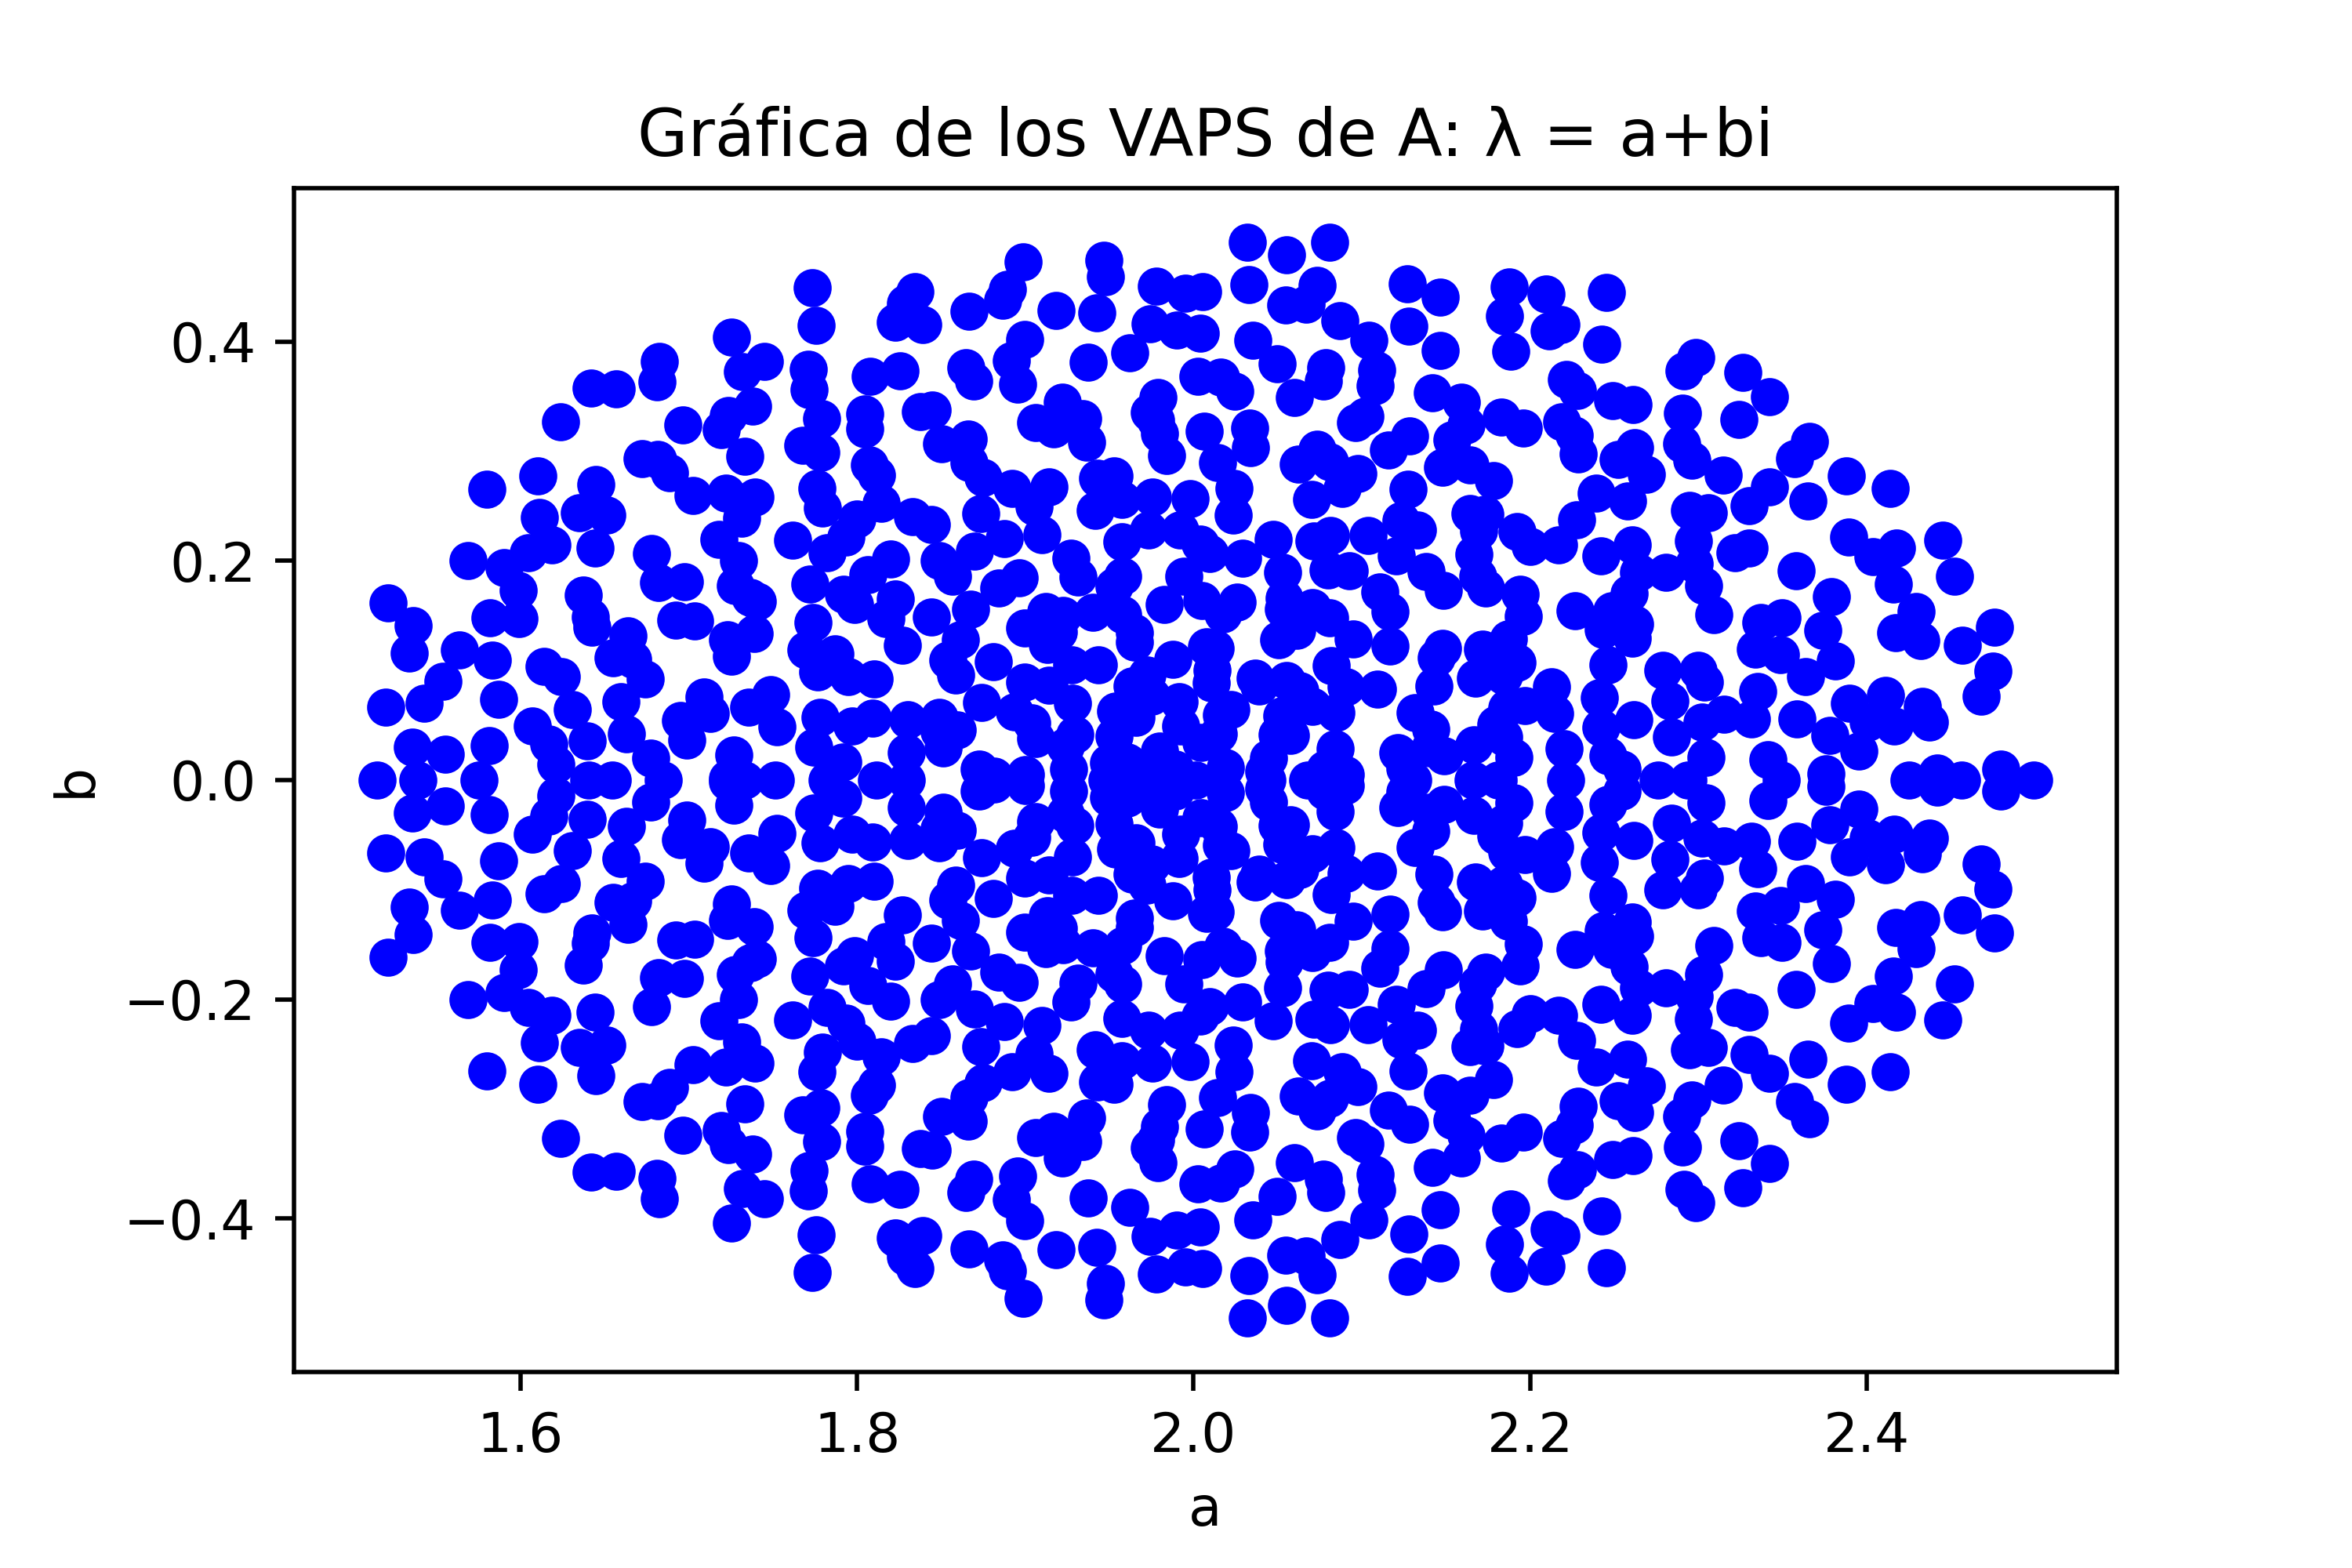
\includegraphics[scale = 0.9]{vaps.png}\\

Esto implica que: $(\forall \lambda \in \lambda(A))(|\lambda-2|\leq \frac{1}{2})$. A continuación generalizaremos el criterio de convergencia según el disco donde se encuentra $\lambda(A)$. Sea $c \in \mathbb{R}$ el centro de la circunferencia y $r \in \mathbb{R}$ el radio de la misma. Utilizando propiedades de complejos y reemplazando por los parámetros mencionados:
\begin{equation}\label{1}
|\lambda-c| \leq r \Leftrightarrow |1-\frac{Re(\lambda)}{c}-i \frac{Im(\lambda)}{c}| \leq \frac{r}{|c|}
\end{equation}
Asumiendo que A es diagonalizable: $A=QDQ^{-1}$ y dada la proposici\'on 6.32 del 
\textit{Iterative methods for sparse linear systems}\cite{itermethods}:
\begin{equation}\label{2}
    \frac{||r^m||_2}{||r^0||_2} \leq k(Q) \max_{\lambda \in \lambda(A)}{|p_m(\lambda)|} \ \forall p_m \in \mathbb{P}_m / p(0)=1
\end{equation}
Donde $k(Q)$ es el número de condición de $Q$. Utilizando el polinomio $p_m(z)=(\frac{-z}{c}+1)$, podemos obtener una cota para el residuo relativo de la siguiente forma:
\begin{equation*}
    |p_m(z)| = |(\frac{-z}{c}+1)^m| = |\frac{-z}{c}+1|^m = |(1-\frac{Re(z)}{c})+i\frac{Im(z)}{c}|^m
\end{equation*}
El cual decrece en función de $m$ $\Leftrightarrow$ $|(1-\frac{Re(z)}{c})-i\frac{Im(z)}{c}| < 1$. Geométricamente esto sucede cuando $z$ se encuentra dentro de $\mathscr{C}(c+0i,c)$ en $\mathbb{C}$. Ahora bien, utilizando este hecho junto a (\ref{1}) y (\ref{2}):
\begin{equation}\label{3}
    \frac{||r^m||_2}{||r^0||_2} \leq k(Q) \max_{\lambda \in \lambda(A)}{|p_m(\lambda)|} = k(Q)\max_{\lambda \in \lambda(A)}{|(1-\frac{Re(\lambda)}{c})-i\frac{Im(\lambda)}{c}|^m} \leq k(Q)\big(\frac{r}{|c|}\big)^m
\end{equation}
Lo cual muestra que la cota de la norma del residuo decrece exponencialmente en función del paso iterativo $m \Leftrightarrow r<|c|$. Es decir, sí $ 0+0i$ no se encuentra dentro de $\mathscr{C}(c,r) $ el método GMRES es convergente.\\

Entonces, como los $\lambda(A)$ están dentro de $\mathscr{C}(2+0i,\frac{1}{2})$, GMRES converge. Este hecho se confirma graficando la evolución de la norma del residuo relativo. Obsérvese que la norma se encuentra siempre debajo de la cota teórica:
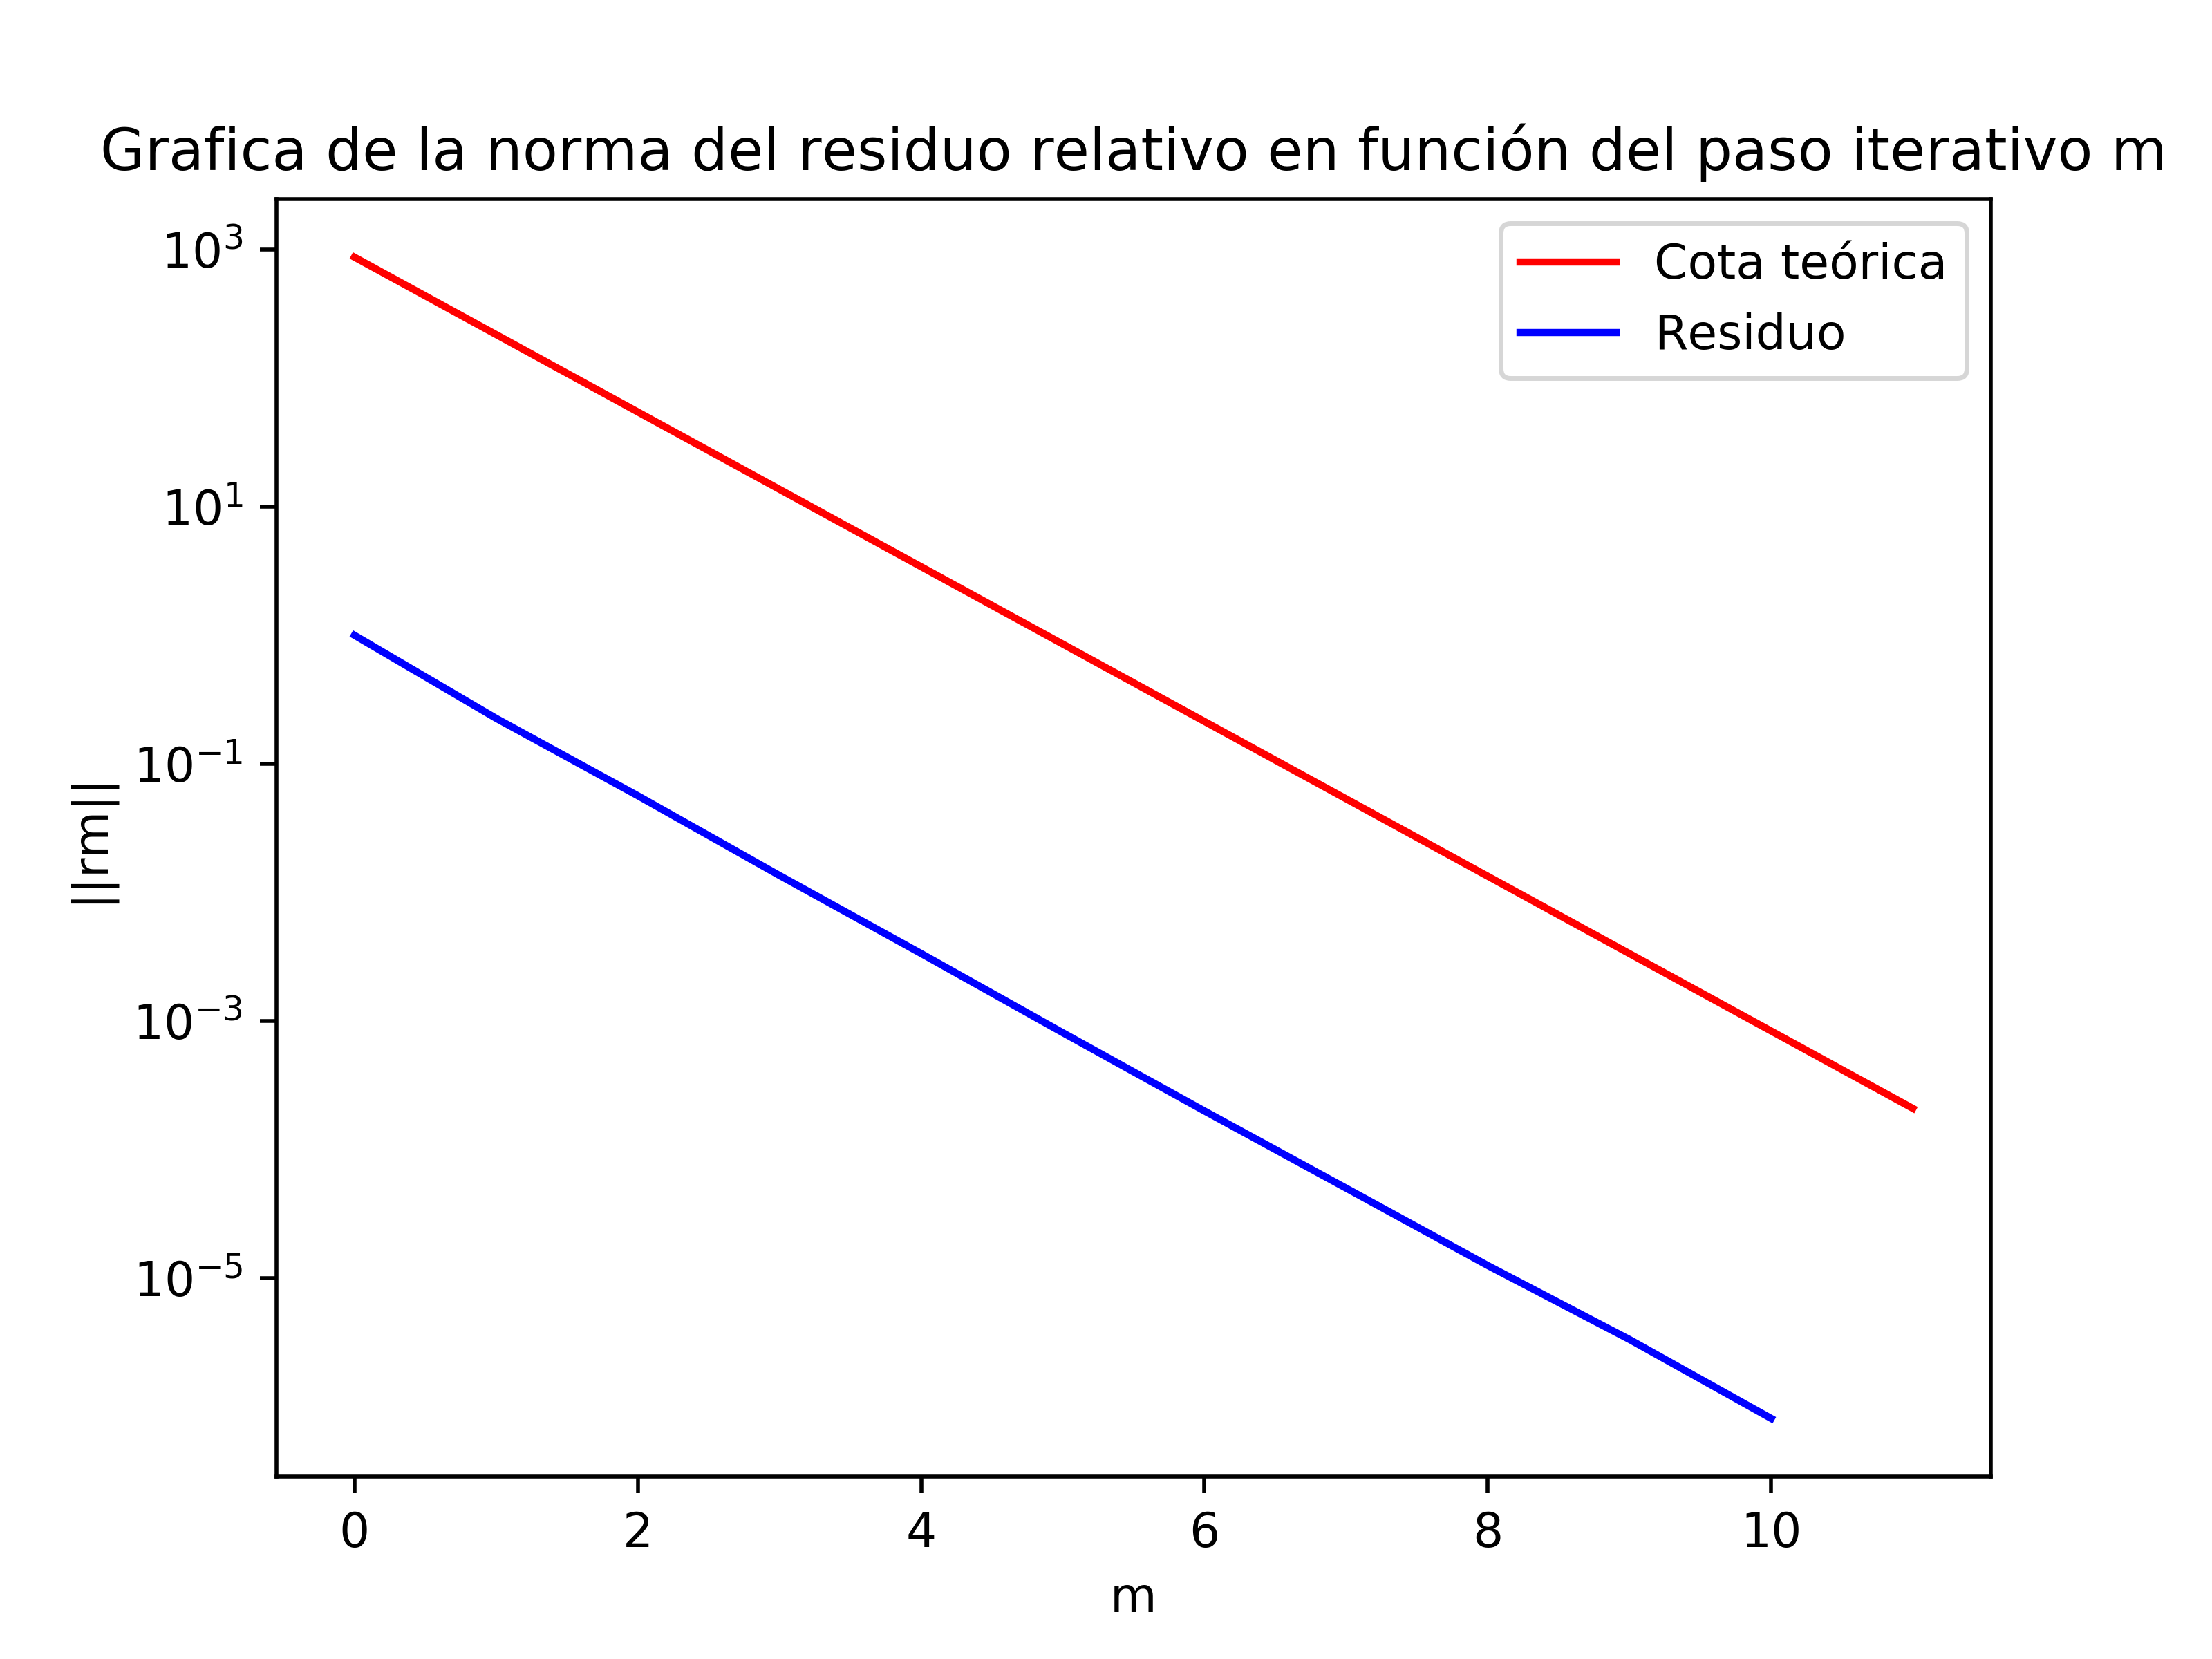
\includegraphics[scale = 0.7]{residuo.png}\\

Adicionalmente, comparamos la solución de nuestra implementación de GMRES con la función $numpy.linalg.solve$, la cual resuelve sistemas lineales utilizando el método directo de descomposición 
LU\cite{linalg} . Observamos que los 6 dígitos decimales más significativos para cada entrada del vector solución $X$ son exactamente iguales para ambos métodos. \\

Alterando los parámetros de la distribución de las entradas no nulas de la matriz $A$ nos encontramos con resultados análogos.\\
Con $A \sim N \Bigg(\mu=\frac{3}{5} \ ,\sigma=\frac{0,5}{\sqrt{1000 \times 0,01}}\Bigg)$ \\
Graficando $\lambda(A$) observamos que están dentro de $\mathscr{C}(\frac{1}{6}+0i,\frac{1}{2})$:
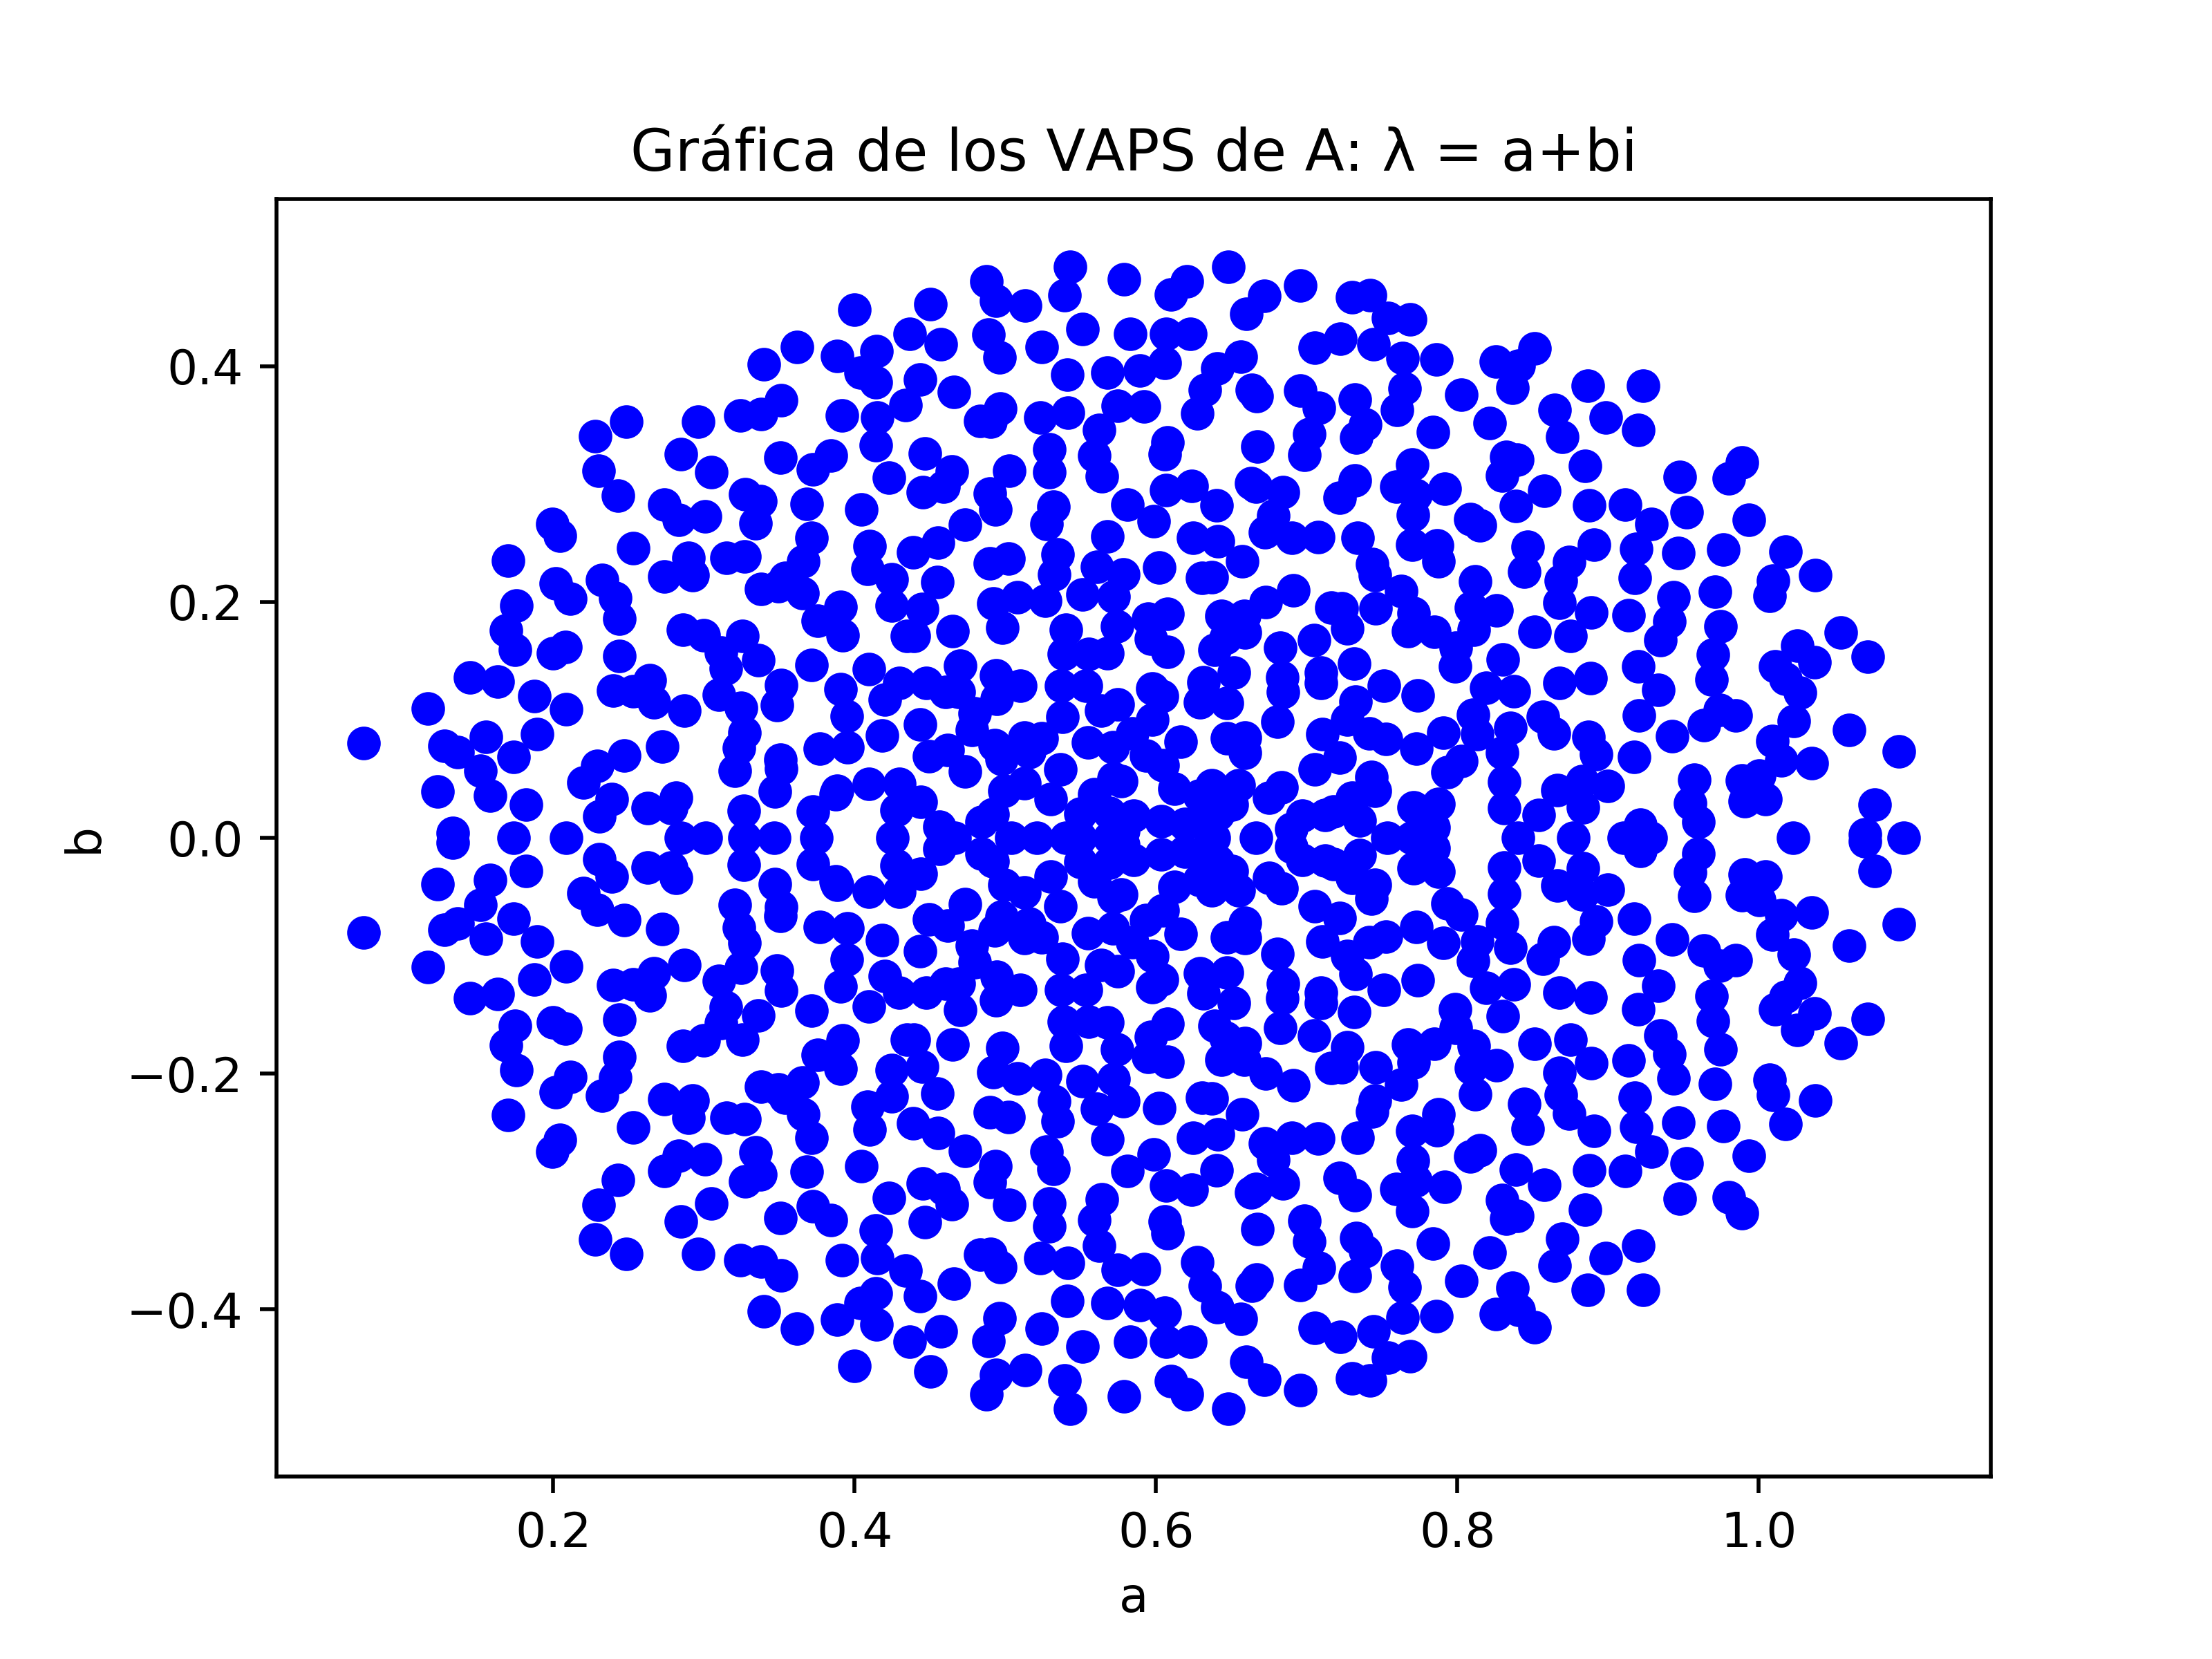
\includegraphics[scale = 0.7]{vaps-5a.png}\\

Es decir, $c=\frac{3}{5}$, $r=\frac{1}{2}$ y $\frac{r}{c} \approx 0,8333$. Por lo que GMRES va a converger. Sin embargo, converger le llevará más iteraciones que en la matriz anterior y de hecho el algoritmo terminará por el tope máximo de iteraciones y no por alcanzar la tolerancia mínima:
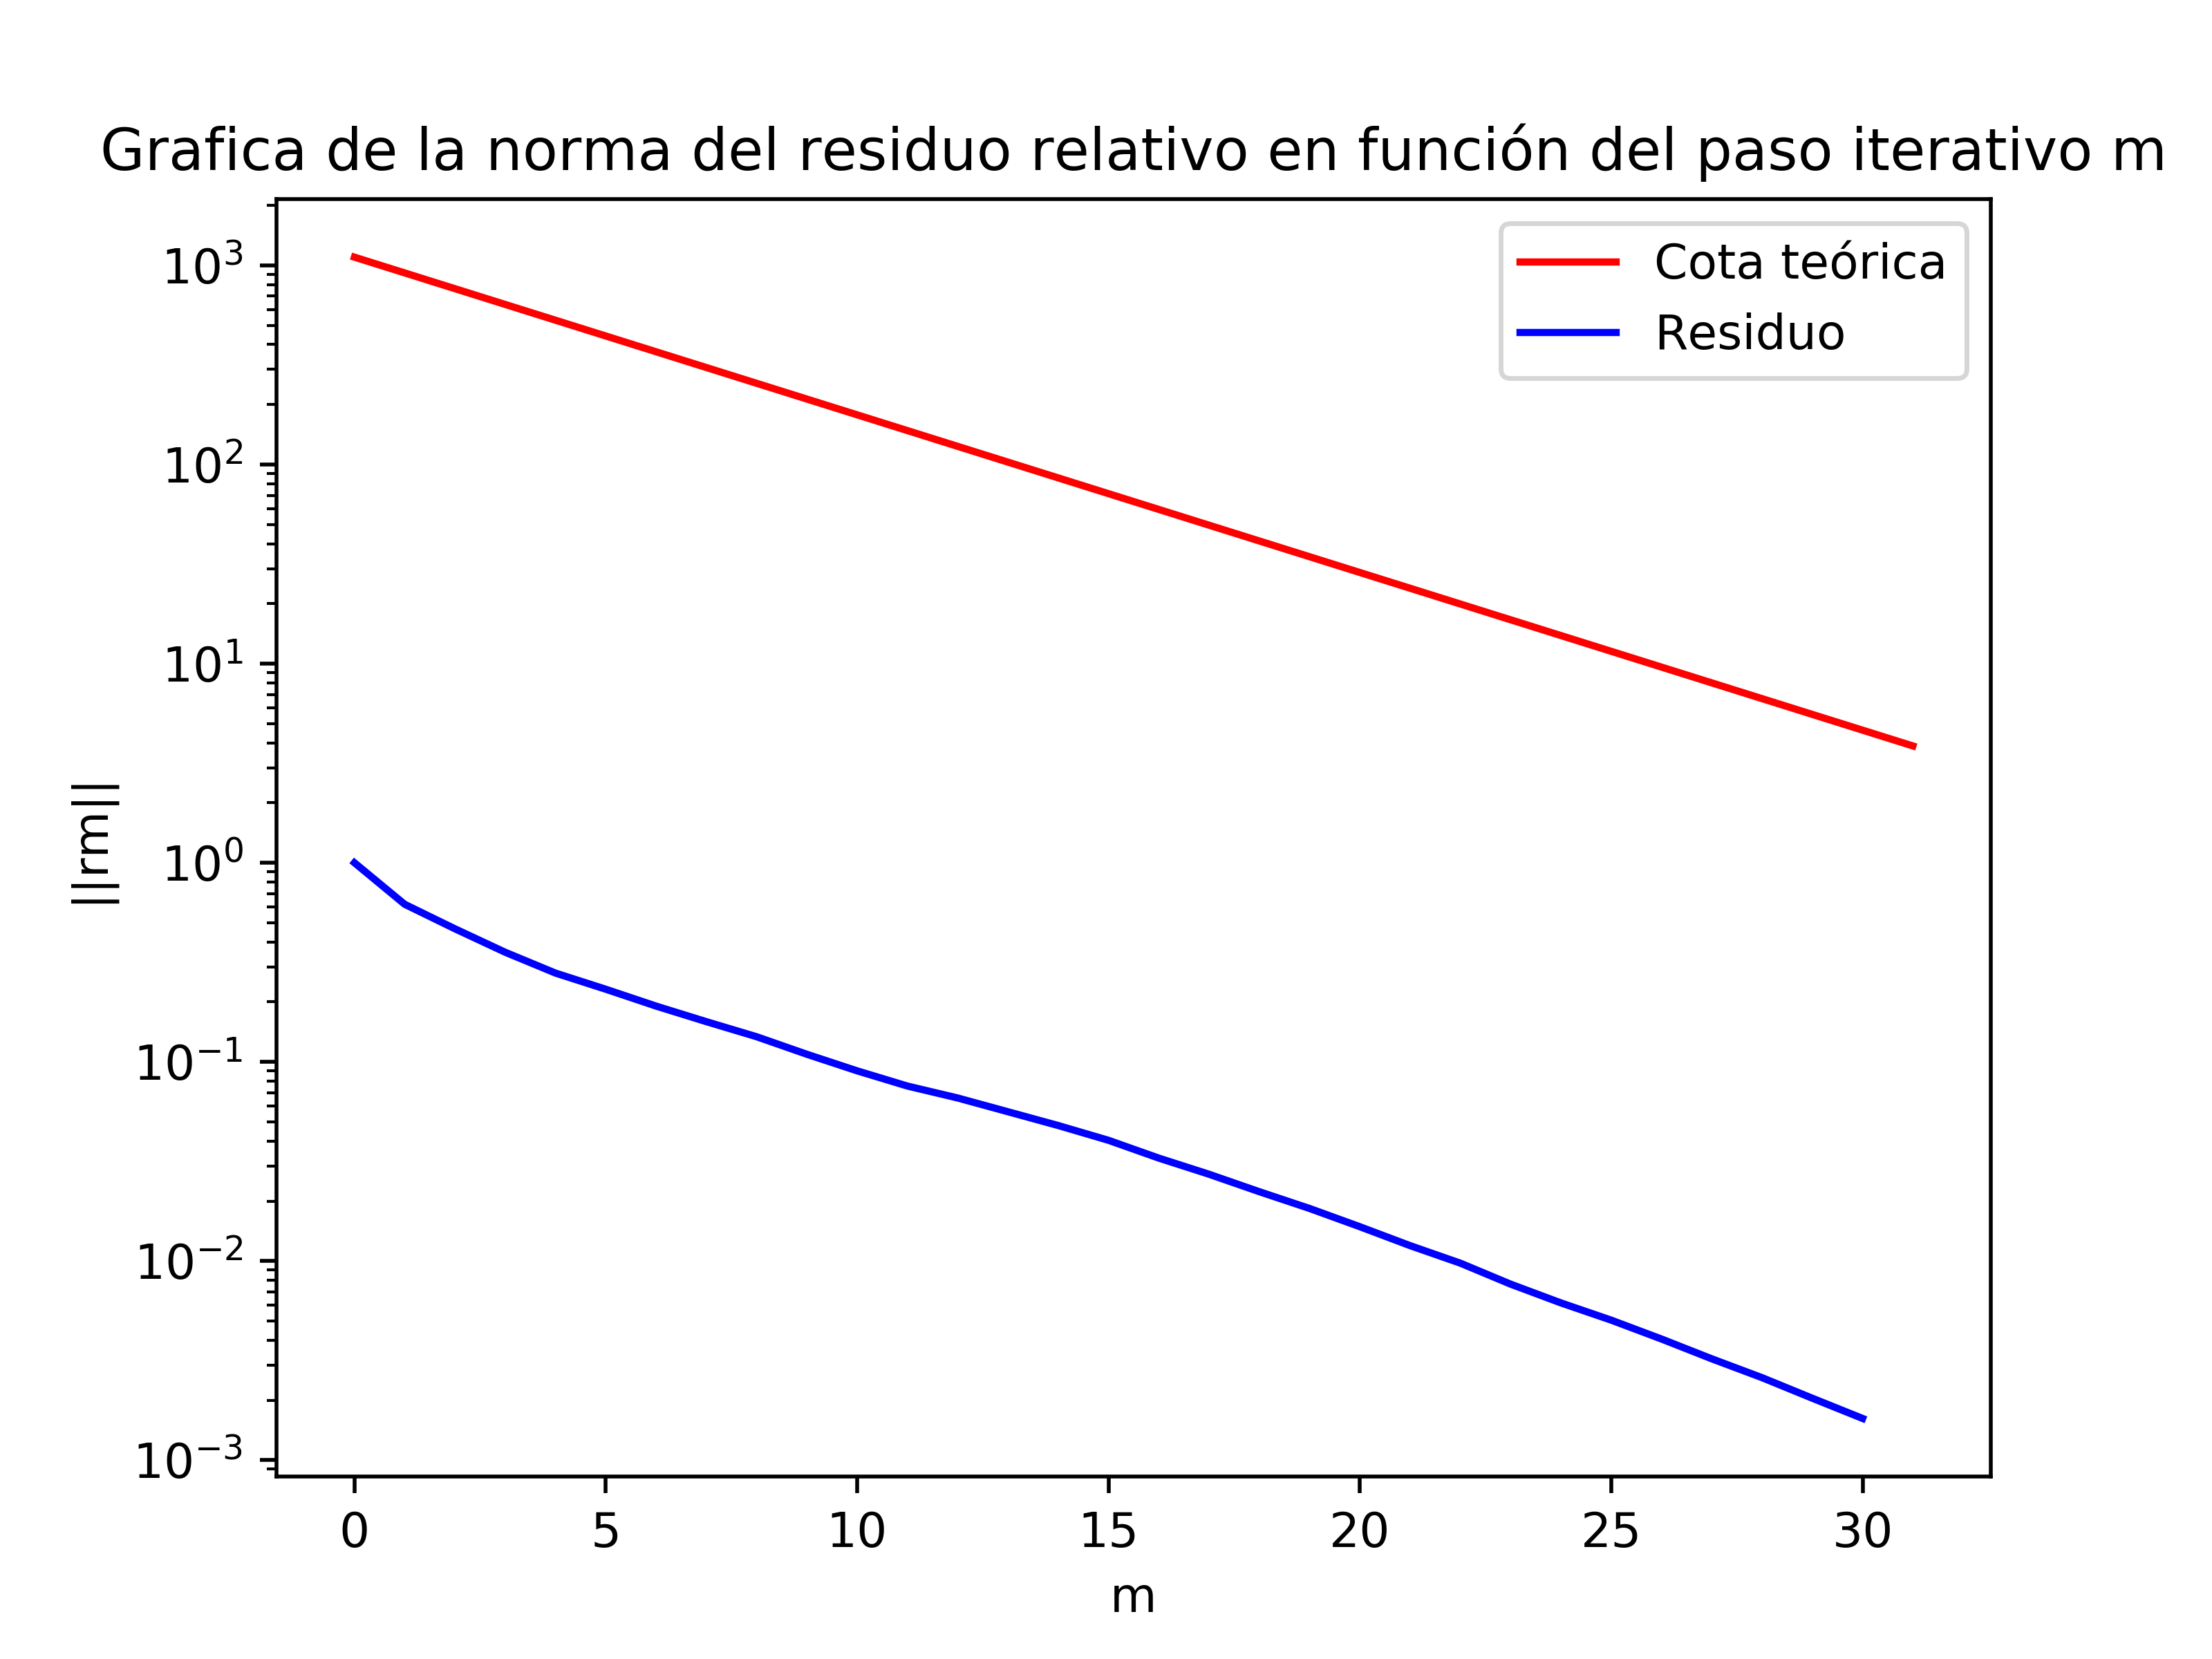
\includegraphics[scale=0.7]{residuo-5a.png}\\

Por último probamos con con $A \sim N \Bigg(\mu=2 \ ,\sigma=\frac{1,9}{\sqrt{1000 \times 0,01}}\Bigg)$. Graficando el disco donde se encuentra $\lambda(A)$ y la evolución del residuo relativo:

\begin{center}
    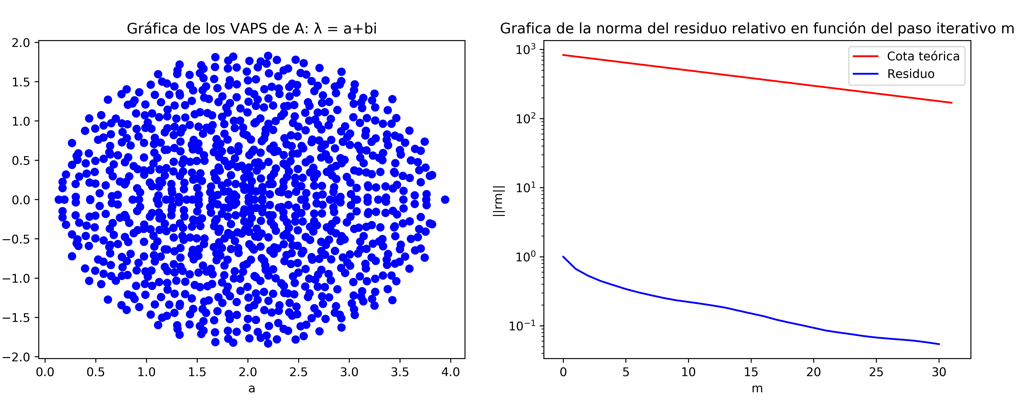
\includegraphics[scale=0.55]{snip2.PNG}\\
\end{center}

Lo cual muestra que (con $r=1,9$, $c=2$ y $\frac{r}{c}=0,95$) GMRES converge pero lentamente. En efecto, el mismo cesa por el máximo de iteraciones y con un error de 5 órdenes mayor a la tolerancia mínima pedida.

Comparando los resultados con $numpy.linalg.solve$ obtenemos soluciones acordes a la norma del error relativo en las últimas dos matrices estudiadas.\\

\subsection{Comparaci\'on de pruebas de tiempo}

Para finalizar el análisis experimental, comparamos los tiempos medios de ejecución de nuestra implementación de GMRES con el comando "contrabarra" de \textit{Octave} en función de la dimensión de la matriz $A$ donde $A \sim N \Bigg(\mu=2,\sigma=\frac{0,5}{\sqrt{n \times d}} \Bigg), \quad d =0.01$

\begin{center}
    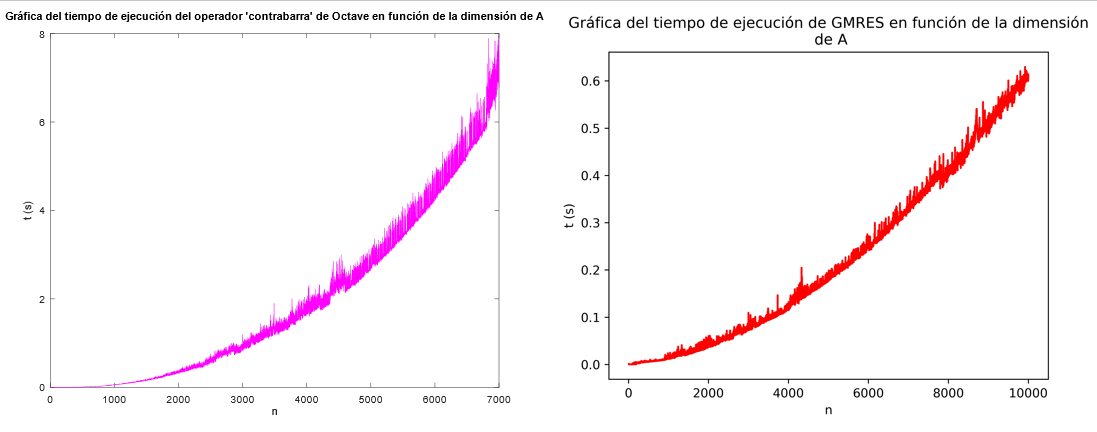
\includegraphics[scale=0.6]{snip.PNG}\\
\end{center}
Las gráficas muestran que la tendencia de crecimiento del tiempo de ejecución medio de GMRES es mucho menor al del comando \textit{“contrabarra”}. Por ejemplo, cuando $n=3000$ nuestra implementación resuelve el sistema, en promedio, aproximadamente 20 veces más rápido que \textit{“contrabarra”}, y cuando $n=7000$ lo resuelve 27 veces más rápido. Nótese como el problema se torna rápidamente irresoluble en la práctica sí solo contásemos con el comando \textit{“contrabarra”}

\section{Conclusiones}\label{Conclusions}
Tras ahondar en la metodología que utiliza GMRES, hemos conseguido implementar el algoritmo y estudiar su comportamiento satisfactoriamente. También encontramos una cota teórica del residuo relativo de este método iterativo, asegurando su convergencia, según $A$.\\
Concluimos que el m\'etodo GMRES resulta extremadamente eficiente para matrices dispersas con distribución normal que cumplen que sus valores propios caen en un disco de centro $c$ y radio $r$ donde el cociente entre c y r es menor a 1. Es decir sí $\frac{r}{|c|} < 1$ GMRES converge y cuanto más pequeño es este cociente mas rápido lo hace. También demostramos que en la pr\'actica, el tiempo de ejecución de GMRES tiene un crecimiento mucho más lento que el comando \textit{“contrabarra”} de \textit{Octave} para resolver $Ax=b$ a medida que la dimensión de $A$ crece para las matrices con las características mencionadas.\\
Esto muestra la importancia del uso de métodos no tradicionales para resolver el problema de hallar un $x$ que cumpla $Ax=b$ dependiendo de las características de $A$. Sí $A$ fuese de dimensión $n=1000000$ no hubiese sido posible resolver el problema $Ax=b$ en un tiempo razonable utilizando el comando \textit{“contrabarra”}. Mientras que el método GMRES lo resuelve en unos pocos segundos sí la matriz $A$ cumple las características deseadas.

%\bibliographystyle{plain}

\bibliographystyle{endm.bst}
\bibliography{biblio}
\end{document}\grid
